\section{Permutationschiffer}
\label{sec:permutations}
En av de tidigare uppfinningarna som kunnat tillämpas inom kryptografin var ett 
redskap som heter \emph{skytale}\index{skytale}.
Den bestod av en pinne av en given tjocklek och en läderrem.
Läderremmen lindades runt pinnen, och därefter skrevs det hemliga meddelandet 
på remmen.
Se bild i \cref{fig:Skytale}.
När meddelandet var klart lindades läderremmen av från pinnen och den fördes 
till mottagaren.
För att kunna läsa texten på läderremmen krävdes att läsaren lindade upp remmen 
på en pinne av samma tjocklek som användes vid skapandet av meddelandet.
Om en pinne av fel diameter används kommer bokstäverna att hamna fel och texten 
blir oläsbar.
\begin{figure*}
	\centering
  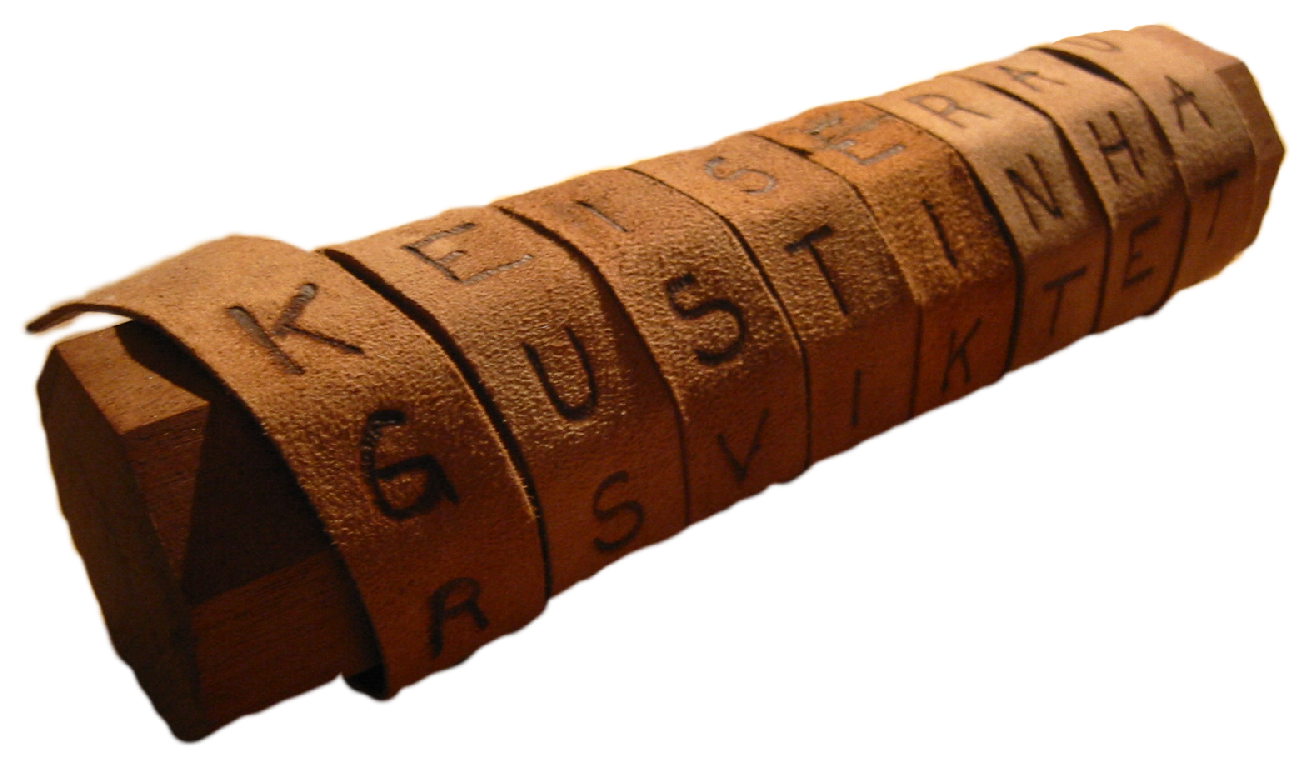
\includegraphics[width=7cm]{figs/skytale.eps}
  \caption{%
    En skytale där texten ''\textsc{keiser augustin \dots}''
		skrivits.
    Bild:~\cite{Wikipedia2011s}.
  }\label{fig:Skytale}
\end{figure*}

Det är dock omdebatterat huruvida denna \enquote{kryptoapparat} uppfanns med 
syfte att vara en kryptoapparat eller bara en metod att lagra meddelanden eller 
en metod att verifiera avsändare~\cite{Kelly1998tmo}.
Hur det än är kan den tillämpas på sådant sätt att det blir ett chiffer, och 
det chiffret tittar vi på här.

Det chiffer som används i kryptoapparaten skytale kan generaliseras enligt 
följande.
Först bestäms bredd och höjd för en rektangel av rutor, där en bokstav ska 
skrivas i varje ruta.
Därefter skrivs texten radvis i rutorna i rektangeln.
Då kan den krypterade texten läsas kolumnvis istället för radvis.
\begin{example}\label{ex:skytaleEnDagIJuni}
	Vi vill kryptera texten \emph{En dag i juni}.
	Vi använder radbredden 7 och kolumnhöjden 2 och markerar tomma rutor med en 
	punkt.
	Vi får då
	\begin{verbatim}
    en_dag_
    i_juni.
  \end{verbatim}
  Kryptotexten blir då \emph{EIN\_\_JDUANGI\_.}.
  För att avkryptera skriver vi bara texten i samma rektangel.
  \begin{verbatim}
    EN_DAG_
    I_JUNI.
  \end{verbatim}
\end{example}
Om vi vill skriva ett längre meddelande används flera rutor.

Denna typ av chiffer kallas för 
\emph{transpositions-}\index{transpositionschiffer} eller 
\emph{permutationschiffer}\footnote{%
	Engelskans \emph{transposition cipher} eller \emph{permutation cipher}.
}\index{permutationschiffer}.

\subsection{Formell definition av permutationschiffer}
Formellt definierar vi ett permutationschiffer enligt följande.
\begin{definition}[Permutationschiffer]\label{def:permutationCipher}\index{permutationschiffer!formell 
    definition}
  Låt \(n\) vara ett positivt heltal och \(A\) ett alfabet.
  Låt också \(\P = \C = A^n\) och låt \(\K\) vara alla möjliga permutationer av 
  mängden \(\{1,\ldots,n\}\).
  För en permutation \(\pi\in \K\) definierar vi
  \begin{align}
    \nonumber
    e_\pi(p_1,\ldots,p_n) = (p_{\pi(1)},\ldots,p_{\pi(n)}),
  \end{align}
  för alla klartexter \(p = (p_1,\ldots,p_n)\in \P\), och
  \begin{align}
    \nonumber
    d_\pi(c_1,\ldots,c_n) = (c_{\pi^{-1}(1)},\ldots,c_{\pi^{-1}(n)}),
  \end{align}
  för alla kryptotexter \(c = (c_1,\ldots,c_n)\in \C\) och där \(\pi^{-1}\) är 
  den inverterade permutationen \(\pi\).
\end{definition}

Låt oss illustrera definitionen genom att tillämpa den på 
\cref{ex:skytaleEnDagIJuni}.
\begin{example}\label{ex:permutationEnDagIJuni}
  Låt \(n = 7\times 2 = 14\).
  Vi låter också permutationen \(\pi\in \K\) definieras enligt 
  \cref{tbl:pi}.
  \begin{table*}
    \caption{%
      Definitionen av permutationen \(\pi\).
    }\label{tbl:pi}
    \centering
    \begin{tabular}{rrrrrrrrrrrrrrr}
      \toprule
      \(i\)       & 1 & 2 & 3 & 4 & 5 & 6 & 7 & 8 & 9 & 10 & 11 & 12 & 13 & 14 
      \\
      \(\pi(i)\)  & 1 & 8 & 2 & 9 & 3 & 10 & 4 & 11 & 5 & 12 & 6 & 13 & 7 & 14 
      \\
      \bottomrule
    \end{tabular}
  \end{table*}
  För att kryptera använder vi \(e_\pi\in \E\).
  Om vi låter \(p = (p_1, \ldots, p_n)\) vara vår klartext \enquote{en dag 
    i juni}, alltså \(p_1 = e, p_2 = n\) och så vidare, får vi att \(c 
    = e_\pi(p) = (p_1, p_8, p_2, p_9, \ldots, p_7, p_{14})\) och således att 
  \(c\) är vår kryptotext \enquote{EIN\_\_JDUANGI\_.}.

  Vi avkrypterar på samma sätt med hjälp av \(\pi^{-1}\).
\end{example}

Om vi vill kryptera ett meddelande som är längre upprepas användningen av 
permutationen, exempelvis om permutationen i \cref{tbl:pi} används 
krypteras 14 tecken åt gången.
Notera dock att en klartext som ska krypteras med denna metod måste vara jämnt 
delbar med storleken för permutationen: 14, 28, \dots, i fallet ovan.
Om detta inte är fallet kan någon form av fyllnadstecken läggas till för att få 
rätt blockstorlek.

Vi ser också ganska omedelbart att antalet möjliga nycklar \(|\K| = {n!}\) 
växer snabbt med antalet bokstäver \(n\) i ett block som permuteras.

\begin{exercise}
  Skapa en permutation av längden \(n = 5\).
  Använd denna för att kryptera en klartext som är minst tio tecken lång.
\end{exercise}
\begin{exercise}
  Byt den resulterande kryptotexten från föregående uppgift med någon annan.
  Börja med att försöka lista ut permutationen som använts vid skapandet av 
  kryptotexten du fått.
  Använd därefter rätt permutation och avkryptera meddelandet.
  Verifiera att du kommit fram till rätt klartext.
\end{exercise}
\begin{exercise}
  Undersök vad som händer vid sammansättning av permutationer.
  Exempelvis om permutationen \(\pi\) i \cref{tbl:pi} appliceras två 
  gånger, eller att två olika permutationer kombineras: spelar det då någon 
  roll i vilken ordning de appliceras?
\end{exercise}

För vidare studier av permutationer, se avsnitt 10.6 och kapitel 21 i Biggs bok 
\emph{Discrete Mathematics}~\cite{Biggs2002dm}.

\begin{exercise}
  Försök att finna en kryptotext \(c\) och två nycklar, \(k\) och \(k^\prime\), 
  sådana att \(d_k(c)\) och \(d_{k^\prime}(c)\) ger tolkningsbara klartexter då 
  permutationschiffret används som kryptosystem.
\end{exercise}
\begin{exercise}
  Varför är det intressant att finna kryptotexter som beroende av nyckel kan 
  avkrypteras till olika läsbara klartexter?
\end{exercise}

